%%%%%%%%%%%%%%%%%%%%%%%%%%%%%%%%%%%%%%%%%%%%%%%%%%%%%%%%%%%%%%%%%%%%%%

\documentclass[useAMS,usenatbib,a4paper]{mn2e}

\voffset=-0.6in

% Packages:
\input psfig.sty
\usepackage{xspace}
\usepackage{graphicx}
\usepackage{amssymb}
\usepackage{amsmath}

% Macros:
% Making life easier
\newcommand{\be}{\begin{equation}}
\newcommand{\ee}{\end{equation}}
\newcommand{\bs}{\begin{split}}
\newcommand{\bea}{\begin{eqnarray}}
\newcommand{\eea}{\end{eqnarray}}

% Useful symbols
\newcommand{\om}{\Omega_m}
\newcommand{\ha}{\frac{1}{2}}
\newcommand{\ahub}{\frac{\dot{a}}{a}}
\newcommand{\ode}{\Omega_{de}}
\newcommand{\Oe}{\Omega_{e}}
\newcommand{\lcdm}{$\Lambda$CDM}
\newcommand{\neff}{N_{\rm eff}}
\newcommand{\hfid}{H^2_{\rm fid}}
\newcommand{\dl}{\delta}
\newcommand{\sumu}{\Sigma m_\nu}
\newcommand{\mnu}{\Sigma m_\nu}
\newcommand{\mpci}{\,{\rm Mpc}^{-1}}

\newcommand{\dataext}{\data_{\rm ext}}
\newcommand{\transferext}{\mathbf{R}_{\rm ext}}
\newcommand{\smat}{\mathbf{S}}
\newcommand{\cmat}{\mathbf{C}^{\epsilon}}
\newcommand{\cmatext}{\mathbf{C}^{\epsilon_{\rm ext}}}
\newcommand{\noisemat}{\mathbf{N}^{\epsilon}}
\newcommand{\noisematext}{\mathbf{N}^{\epsilon_{\rm ext}}}
\newcommand{\noisematinv}{\left(\noisemat\right)^{-1}}
\newcommand{\noisemattransfer}{\tilde{\mathbf{N}}^{\epsilon}}
\newcommand{\noisemattransferext}{\tilde{\mathbf{N}}^{\epsilon_{\rm ext}}}
\newcommand{\noisemattransferinv}{\left(\tilde{\mathbf{N}}^{\epsilon}\right)^{-1}}
\newcommand{\noisemattransferextinv}{\left(\tilde{\mathbf{N}}^{\epsilon_{\rm ext}}\right)^{-1}}

% Macros
\newcommand{\half}{\frac{1}{2}}
\newcommand{\rhocrit}{\rho_{\rm crit}}
\newcommand{\rvir}{r_{\rm vir}}
\newcommand{\mvir}{m_{\rm vir}}
\newcommand{\kv}{\mathbf{k}}
\newcommand{\xv}{\mathbf{x}}
\newcommand{\mv}{\mathbf{m}}
\newcommand{\muv}{\bm \mu}
\newcommand{\hmsun}{h^{-1}M_{\odot}}
\newcommand{\hmpc}{h^{-1}Mpc}
\newcommand{\hgpc}{h^{-1}{\rm Gpc}}

%%% "Data" - i.e., the observed CMB temperature map
\newcommand{\data}{\mathbf{d}}
%%% Parameters: gravitational potential
\newcommand{\Pot}{\Phi}
\newcommand{\Potvector}{\boldsymbol{\Pot}}
%%% "Signal" - i.e., zero-noise CMB temperature
\newcommand{\signal}{\mathbf{s}}
%%% "noise" - i.e., the pixel noise realization
\newcommand{\noise}{\mathbf{n}}
%%% Transfer function relating the 3D gravitational potential to the
%%% 2D CMB temperature (or other) map
\newcommand{\transfer}{\mathsf{R}}
%%% Signal and noise covariance matrices
\newcommand{\Smat}{\mathsf{S}}
\newcommand{\Nmat}{\mathsf{N}}
\newcommand{\Psimat}{\mathsf{\Psi}}
\newcommand{\Sigmamat}{\mathsf{\Sigma}}
\newcommand{\Cmat}{\mathsf{C}}
%%% Gravitational potential represented as a vector of "voxels" or similar
\newcommand{\gravpot}{\bm \Psi}
%%% Normal (Gaussian) distribution
\newcommand{\normdist}{\mathcal{N}}
%%% Probability theory
\newcommand{\pr}{{\rm Pr}}


%%%%%%%%%%%%%%%%%%%%%%%%%%%%%%%%%%%%%%%%%%%%%%%%%%%%%%%%%%%%%%%%%%%%%%

\title[Topological Non-Gaussianity Tests]
{The Music of the Sphere: Topological Tests of Non-Gaussianity}

\author[Blandford et al.]{%
    Roger~D.~Blandford,$^{1}$\thanks{\rdbemail}
    Philip~J.~Marshall,$^{1}$
    Laurence Perrault Levasseur$^{1}$
    \medskip\\
    $^1$\kipac
}


%%%%%%%%%%%%%%%%%%%%%%%%%%%%%%%%%%%%%%%%%%%%%%%%%%%%%%%%%%%%%%%%%%%%%%

\begin{document}

\date{to be submitted to arxiv}
\pagerange{\pageref{firstpage}--\pageref{lastpage}}\pubyear{2015}

\maketitle

\label{firstpage}

%%%%%%%%%%%%%%%%%%%%%%%%%%%%%%%%%%%%%%%%%%%%%%%%%%%%%%%%%%%%%%%%%%%%%%

\begin{abstract}

Abstract goes here.

\end{abstract}

% Full list of options at http://www.journals.uchicago.edu/ApJ/instruct.key.html

\begin{keywords}
  cosmology
\end{keywords}

\setcounter{footnote}{1}

%%%%%%%%%%%%%%%%%%%%%%%%%%%%%%%%%%%%%%%%%%%%%%%%%%%%%%%%%%%%%%%%%%%%%%

\section{Introduction}

Motivation.

Questions to be answered.

This paper is organized as follows.

%%%%%%%%%%%%%%%%%%%%%%%%%%%%%%%%%%%%%%%%%%%%%%%%%%%%%%%%%%%%%%%%%%%%%%

\section{Nesting of Equipotential Lines on the Sphere}

Analyze the potential on the cosmic photosphere ($x=1$) in a way that
will generalize to the 3D potential in the sphere. The $\ell=0$ term
is just a constant and, although necessary for the expansion we have
just described, can be ignored here.  The $\ell=1$ surface potential
$\Phi(\ell,\theta,\phi)$ develops a single simple minimum (henceforth
designated as $L_0$) and single simple maximum (henceforth designated
by $H_0$). These are the global  minimum and maximum; additional
higher and lower minima and maxima will be designated $L_i$ and $H_i$
respectively in the order in which they appear.

\subsection{Classification of saddles}

Now gradually increase $\ell$. One contour develops a simple
\emph{saddle}\footnote{We are interested in \emph{non-degenerate}
critical points and exclude \emph{degenerate} extrema like
\emph{monkey saddles} which are structurally unstable and unfold into
simple extrema under a small perturbation.} and an extremum
simultaneously, becoming a \emph{separatrix}. This contour divides the
sphere into an \emph{inside} containing $L_0$ and \emph{outside}
containing $H_0$. When the new extremum is a $L$ lying outside the
contour, the separatrix/saddle combination has the shape of an
infinity symbol and called a \emph{lemniscate}, denoted by $X$; when
it is a $H$ lying inside the contour, the separatrix/saddle
combination has the shape of a pinched annulus and is called a
\emph{lima\c con}, denoted by $K$ (Fig.~3). As $\ell$ is further
increased, the two stationary points separate and the smaller loop
grows in size.\footnote{Note that had we associated the interior with
$H_0$, a given contour would have had the opposite identification.}
Further increasing $\ell$ will lead to the \emph{creation} of new
separatrices. These may be located between two existing separatrices
or out of a contour encircling a $L$ or a $H$.  Occasionally, the
inverse process - \emph{annihilation} will occur. If we designate the
total  number of maxima, minima, saddles, lemniscates and lima\c cons
by $N_H,N_L,N_S,N_X,N_K$, respectively, then clearly
$N_S=N_X+N_K=N_H+N_L-2$.

\begin{figure}
\centering
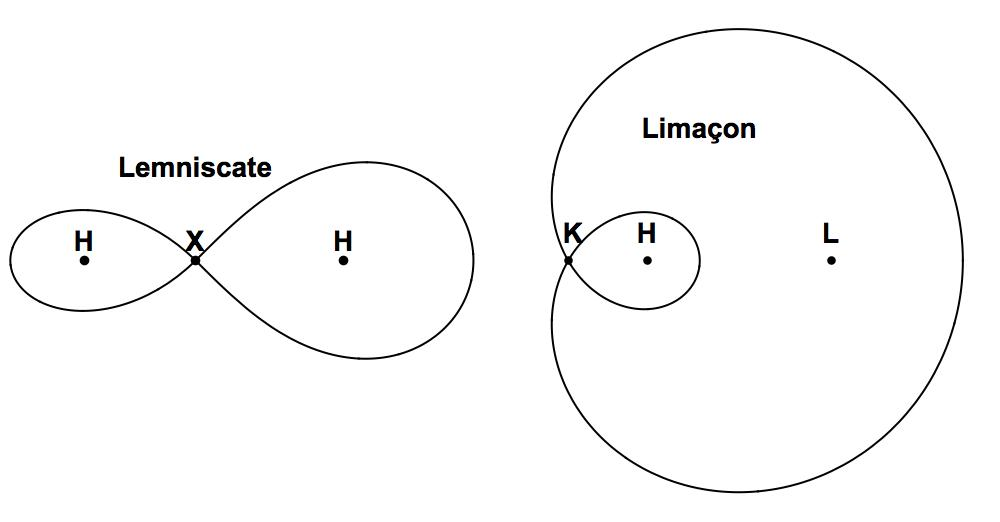
\includegraphics[width=0.9\linewidth]{figures/fig3.jpg}
\caption{Two elementary types of saddle as characterized by the shape of the separatrix -- the equipotential passing through the saddle. The lemniscate, or $X$-saddle, is accompanied by two maxima $H$ , as here, or two minima, $L$. The \emph X may be created or annihilated with an extremum by growing or shrinking either of the closed loops that passes through it. The lima\c con, or $K$-saddle, is accompanied by a $H$ as here (or a $L$) and a $L$ as here (or a $H$). It can be create or annihilated only with one of the two accompanying extrema, in this case the $H$, so long as the contour does not expand and pass around the back of the sphere.}
\end{figure}

\subsection{Tree representation}
The nesting of all of the separatrices suffices to describe the nesting of all of the equipotentials. It is convenient to represent this nesting using a type of \emph{directed graph} or \emph{tree} representation. A simple example of a nesting is shown in Fig.~4a and the associated tree is presented in Fig.~4b.  The tree comprises \emph{nodes} or \emph{vertices}, each with three \emph{branches} or \emph{edges}, each corresponding to a separatrix and \emph{leaves} at the end of a branch corresponding to local extrema. There is only one path connecting any two leaves and no circuits, consistent with the usual definition of a tree. However, our tree has some novel features including growth.  We start with $\ell=1$ and a single branch from the $L$ (the \emph{root}) to the $H$ (the \emph{apex}). We let the vertical height of the branch be the potential difference between the two extrema. as we increase $\ell$, new node-leaf (saddle-extremum) pairs appear and we locate them with ordinates corresponding to their respective potentials. The $X$- and $K$-saddles are easily distinguished. The pre-existing nodes and leaves will also move and occasionally they may disappear; they may also pass through each other on a branch when their heights coincide. The horizontal separation of the nodes and leaves is adjusted to ensure that there are no crossovers; it has no quantitative significance. This description of the equipotentials is essentially topological and pays no attention to the actual location of the contours.

\begin{figure}
\centering
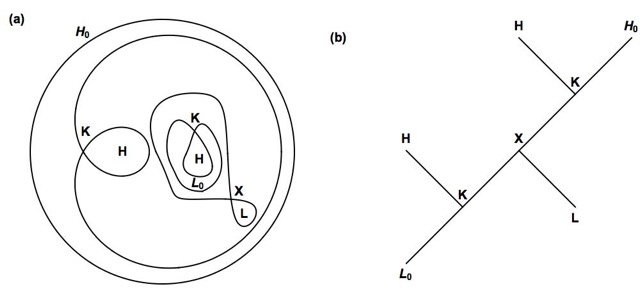
\includegraphics[width=0.9\linewidth]{figures/fig4.jpg}
\caption{(a) Nesting of separatrices  exhibited within a circle created by puncturing the sphere at the global maximum and stretching the surface to lie on a plane so that the circumference is identified with a single point. b) Same separatrices displayed on a sphere. (c) Tree representation of this nesting. The designation of the saddles $X$, $K$ and the extrema, $H$, $L$, is redundant and can be dropped. The numbers designate the order in which the extrema appear as $\ell$ is increased.}
\end{figure}

\subsection{Stationary points}
Finding all the stationary points can be difficult.  The simplest approach is to set $\nabla_2\Phi=\Phi_{ij}=\{\partial\Phi/\partial{\hat\theta},\partial\Phi/\partial{\hat\phi}\}$ to zero, using the identity $P_\ell'(\mu)=\ell[P_{\ell-1}(\mu)-\mu P_\ell(\mu)]/(1-\mu^2)$ and differentiating the sums in Eq.~2. This defines two families of curves and the stationary points are located where they intersect. New stationary points appear when these curves first touch.\footnote{In the language of catastrophe theory , this is a fold catastrophe.} An alternative method, which works well, is to find local minima of $|\nabla_2\Phi|^2$.

\subsection{Curvature maps}
There is another way to discuss the critical points and this is to evaluate the Hessian matrix
\begin{equation}
H_{ij}=\Phi_{,{\hat i}{\hat j}}
\end{equation}
where the derivatives are with respect to $\hat\theta$, $\hat\phi$. It is straightforward to compute the two real eigenvalues which represent the principle curvatures. We can then designate $L$-zones, where they are both negative, $H$-zones, where they are both positive and $S$-zones  where they have opposite signs. (We can further subdivide these zones dependent upon which eigenvalue has the larger absolute value but will not do this here.)  As can be seen in Fig.~5, $H$ and $L $ zones have common boundaries with $S$, where one eigenvalue changes sign and touch at points where both eigenvalues simultaneously pass through zero.  New saddle-extremum pairs are created at saddle boundaries and then quickly separate into their respective zones. This provides an alternate means to locate new separatrices. Individual curvature zones can contain multiple or no stationary points.

\begin{figure}
\centering
%\includegraphics[width=0.9\linewidth]{figures/fig5.jpg}
\caption{Division of sphere into curvature zones. The $L$-zone is denoted in blue, the $H$-zone in red and the $S$-zone in purple. Also shown are the lines where the two components of $\nabla\Phi$ vanish. Their intersections correspond to stationary points.}
\end{figure}

\subsection{Curve of growth}
The number of extrema, measured by the number of saddles $N_S$ increases with $\ell$. The manner in which it does this is dictated by the slope of the power spectrum of potential fluctuations $P_{\bf k}$ though not it's amplitude. We have focused on the inverse cube case because this is close to the inferred initial spectrum and remains valid around recombination up to $\ell\sim30$. (It is also the spectrum for the temperature perturbations because the gravitational redshift is the dominant effect in the \emph{Sachs-Wolfe} regime.) General scaling arguments suggest that as long as $P(k)\propto k^{n-4}$ for fixed $n$ then the expectation in the number of saddles counted when all $N_S(\ell)$ is given asymptotically by $K(n)\ell^2$ as $\ell\rightarrow\infty$ where $K$ can be estimated using a large number of  trials. The variance in the actual value of $K$ for finite $\ell$ can also be computed. We can also apply this approach directly to the temperature fluctuations assuming the inferred fluctuation spectrum inferred by more conventional methods. This will be demonstrated in a subsequent publication but is no more than a consistency check.

\subsection{Gaussianity}
We have considered several ways to classify the extrema and the results can be used to check on the Gaussianity of the distribution of Fourier components. For example, if the distributions of the Fourier coefficients were systematically skewed, then we would expect differences in the numbers of $L$ and $H$ and the areas of the corresponding zones. More subtle tests are possible using the branching of the trees. These will be considered elsewhere and compared with the observations.


%%%%%%%%%%%%%%%%%%%%%%%%%%%%%%%%%%%%%%%%%%%%%%%%%%%%%%%%%%%%%%%%%%%%%%

\section{Nesting of Equipotential Surfaces in the Sphere}

%%%%%%%%%%%%%%%%%%%%%%%%%%%%%%%%%%%%%%%%%%%%%%%%%%%%%%%%%%%%%%%%%%%%%%

\section{Discussion}

%%%%%%%%%%%%%%%%%%%%%%%%%%%%%%%%%%%%%%%%%%%%%%%%%%%%%%%%%%%%%%%%%%%%%%

\bibliographystyle{apj}
\bibliography{references}

%%%%%%%%%%%%%%%%%%%%%%%%%%%%%%%%%%%%%%%%%%%%%%%%%%%%%%%%%%%%%%%%%%%%%%

\end{document}

%%%%%%%%%%%%%%%%%%%%%%%%%%%%%%%%%%%%%%%%%%%%%%%%%%%%%%%%%%%%%%%%%%%%%%
